\documentclass[tikz,border=10px, convert={density=300,outext=.png}]{standalone}
\usepackage{tikz}
\usetikzlibrary{shapes.geometric, arrows, positioning, fit, calc, backgrounds}

\begin{document}

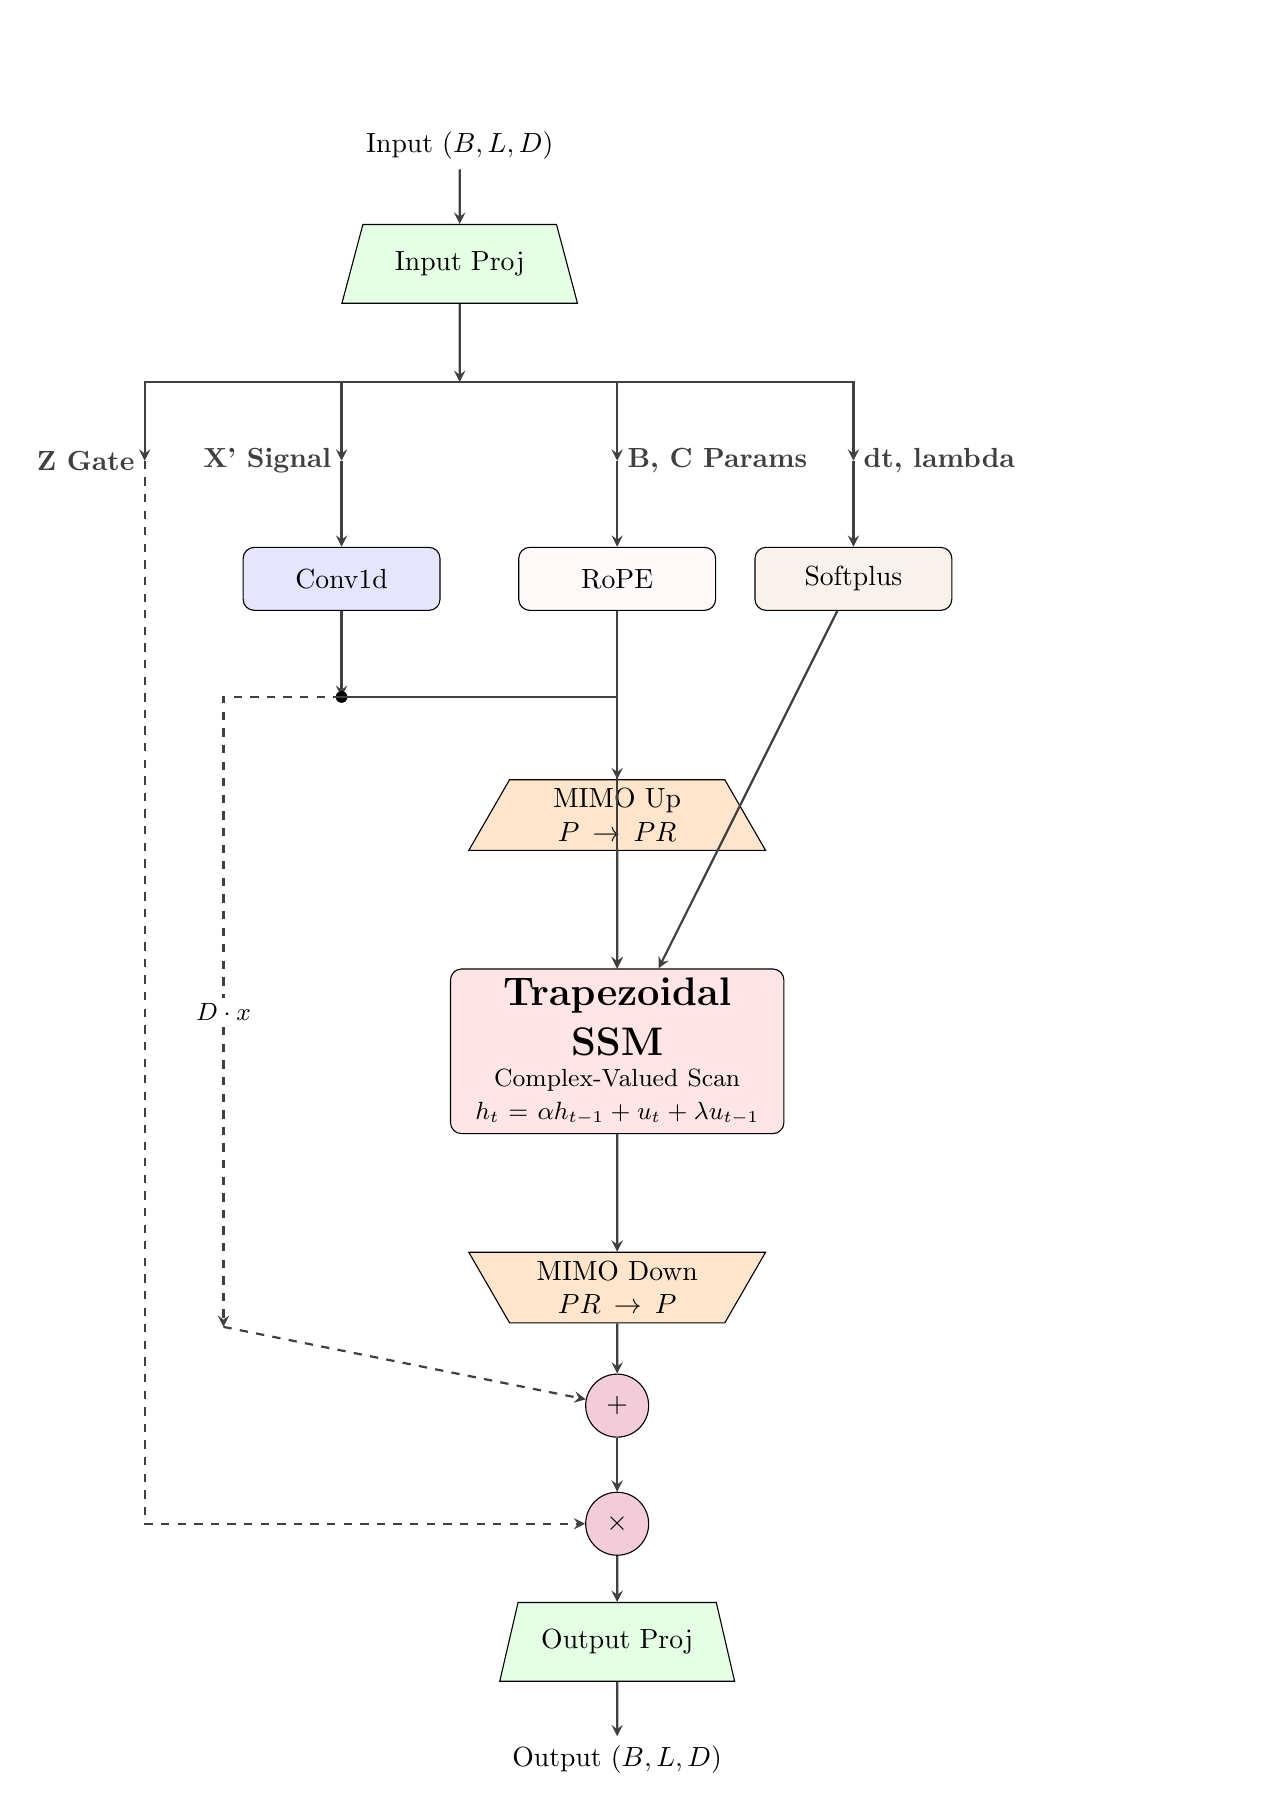
\begin{tikzpicture}[
    node distance=1.5cm,
    block/.style={trapezium, trapezium stretches=true, draw, fill=green!10, minimum width=3cm, minimum height=1cm, text centered, inner sep=0pt},
    rect/.style={rectangle, draw, rounded corners, fill=blue!5, minimum width=2.5cm, minimum height=0.8cm, text centered},
    op/.style={circle, draw, fill=purple!20, minimum size=0.8cm, inner sep=0pt, text centered},
    conn/.style={->, >=stealth, thick, darkgray},
    branch/.style={circle, fill, inner sep=1.5pt}
]

% White Background to prevent transparency issues
\path [fill=white] (-5, -20.5) rectangle (10, 1.5);

% ==================== VERTICAL DATA FLOW ====================

\node (in) at (0, 0) {Input $(B, L, D)$};
\node[block] (proj) at (0, -1.5) {Input Proj};
\draw[conn] (in) -- (proj);

% Split
\coordinate (split) at (0, -3);
\draw[conn] (proj) -- (split);

% Branches
\node (b_z) at (-4, -3) {};
\node (b_x) at (-1.5, -3) {};
\node (b_bc) at (2, -3) {};
\node (b_dt) at (5, -3) {};

\draw[conn] (split) -- (b_z.center) -- node[left, yshift=-0.5cm] {\textbf{Z Gate}} ++(0, -1) coordinate (z_start);
\draw[conn] (split) -- (b_x.center) -- node[left, yshift=-0.5cm] {\textbf{X' Signal}} ++(0, -1) coordinate (x_start);
\draw[conn] (split) -- (b_bc.center) -- node[right, yshift=-0.5cm] {\textbf{B, C Params}} ++(0, -1) coordinate (bc_start);
\draw[conn] (split) -- (b_dt.center) -- node[right, yshift=-0.5cm] {\textbf{dt, lambda}} ++(0, -1) coordinate (dt_start);

% Components Row 1
\node[rect, fill=blue!10] (conv) at (-1.5, -5.5) {Conv1d};
\draw[conn] (x_start) -- (conv);

\node[rect, fill=pink!10] (rope) at (2, -5.5) {RoPE};
\draw[conn] (bc_start) -- (rope);

\node[rect, fill=brown!10] (soft) at (5, -5.5) {Softplus};
\draw[conn] (dt_start) -- (soft);

% Processed X Split for D-Skip
\coordinate (x_proc) at (-1.5, -7);
\draw[conn] (conv) -- (x_proc);
\node[branch] at (x_proc) {};

% MIMO Up
\node[trapezium, draw, fill=orange!20, minimum width=3cm, text width=2.5cm, align=center] (mimo_up) at (2, -8.5) {MIMO Up\\$P \to PR$};
\draw[conn] (x_proc) -| (mimo_up);

% D-Skip Path (Left side)
\draw[conn, dashed] (x_proc) -- (-3, -7) -- (-3, -15) coordinate (d_skip_end);
\node[fill=white, inner sep=2pt] at (-3, -11) {\small $D \cdot x$};


% SSM Input Merge
% All go into SSM
\node[rectangle, draw, fill=red!10, text width=4cm, minimum height=2cm, align=center, rounded corners] (ssm) at (2, -11.5) {\Large \textbf{Trapezoidal SSM}\\ \small Complex-Valued Scan\\ \small $h_t = \alpha h_{t-1} + u_t + \lambda u_{t-1}$};

\draw[conn] (mimo_up) -- (ssm);
\draw[conn] (rope) -- (ssm);
\draw[conn] (soft) -- (ssm);

% MIMO Down
\node[trapezium, shape border rotate=180, draw, fill=orange!20, minimum width=3cm, text width=2.5cm, align=center] (mimo_down) at (2, -14.5) {MIMO Down\\$PR \to P$};
\draw[conn] (ssm) -- (mimo_down);

% Add D-Skip
\node[op] (add) at (2, -16) {$+$};
\draw[conn] (mimo_down) -- (add);
\draw[conn, dashed] (d_skip_end) -- (add);

% Gate Multiply
\node[op] (mult) at (2, -17.5) {$\times$};
\draw[conn] (add) -- (mult);

% Z Path connection
\draw[conn, dashed] (z_start) -- (-4, -17.5) -- (mult);

% Output Proj
\node[block] (out_proj) at (2, -19) {Output Proj};
\draw[conn] (mult) -- (out_proj);

% Output
\node (out) at (2, -20.5) {Output $(B, L, D)$};
\draw[conn] (out_proj) -- (out);

\end{tikzpicture}
\end{document}
